\begin{frame}
 \textbf{Objectives with the use of Kalman filte}
 \begin{itemize}
 	\item VF-LQR controller needs an estimate of the consumer demand.
 	\item The optimal estimator is the \textbf{Kalman Filter}.
 	\item Recursively finds optimal Kalman gain.
 	\item Kalman filter is also very interesting when from a leakage detection POV.  
 \end{itemize}
\end{frame}

	\begin{frame}{Water consumption data}
		\begin{itemize}
			\item Data of consumption pattern over a 35 day period obtained by CSK.  
		\end{itemize}
			 \begin{figure}[h!]
			\centering
			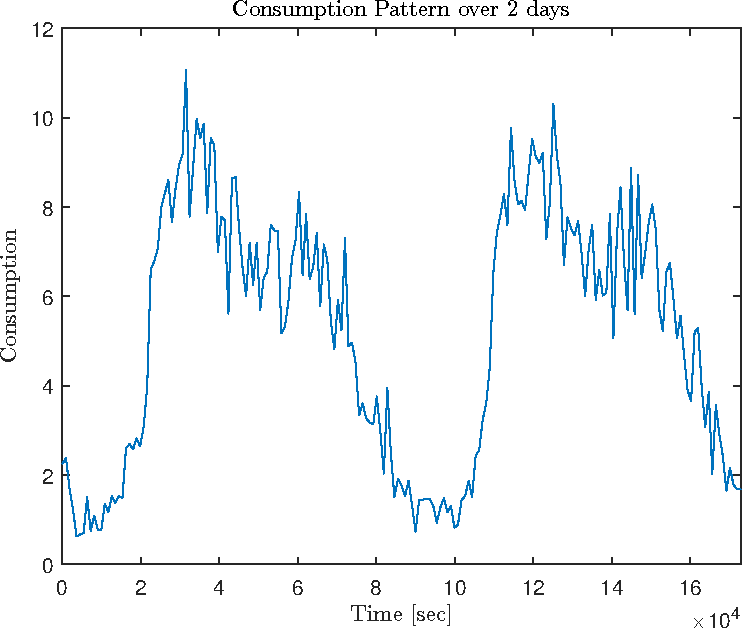
\includegraphics[width=0.6\textwidth]{Topics/KalmanEstimator/Graphics/ConsumptionPattern.pdf}
			\caption{Consumption pattern over two days}
			\label{fig:Consumption_Pattern}
		\end{figure}
	\end{frame}
	
	\begin{frame}{FFT of consumption pattern}
		\begin{itemize}
			\item Frequency analysis of the data. 
		\end{itemize}
	
		 \begin{figure}[h!]
			\centering
			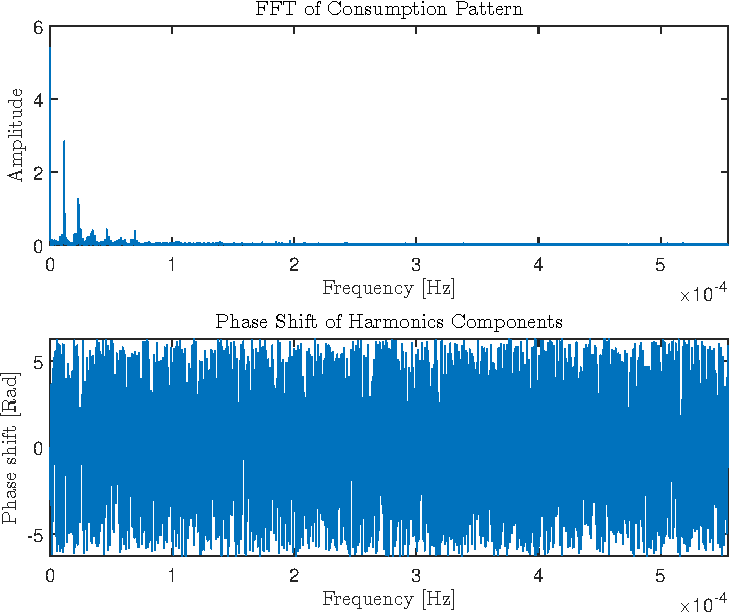
\includegraphics[width=0.6\textwidth]{Topics/KalmanEstimator/Graphics/FFT.pdf}
			\caption{Consumption pattern over two days}
			\label{fig:FFT_Consumption_Patter}
		\end{figure}
	
	\begin{itemize}
		\item Highest frequency contents at periods: DC, 24.05h, 12.03h, 8.02h and 5.99h. 
	\end{itemize}

	\end{frame}

%%%%%%%%%%%%%%%%%
	\begin{frame}{Approximation of consumption}
		
	\begin{itemize}
		\item Fourth order Fourier approximation of consumer demand:
	\end{itemize}
		
	\begin{equation} \label{eq:4th_order_approx}
		\begin{split}
			d_c(t) \approx& k_0 + k_1 cos(\omega_1 t + \phi_1) + k_2 cos(\omega_2 t + \phi_2)\\
			&+ k_3 cos(3\omega_3 t + \phi_3) + k_4 cos(4\omega_4 t + \phi_4)
		\end{split}
	\end{equation}

	\begin{itemize}
		\item We wish to model \ref{eq:4th_order_approx} as a state space model:
	\end{itemize}
		
			\begin{equation*}
			\begin{split}
				\dot{x}=Ax\\
				y=Cx
			\end{split}
		\end{equation*}	
	\end{frame}
%%%%%%%%%%%%%%%%%%%%%%%
\begin{frame}{State space representation}
	\begin{itemize}
		\item Need to represent the evolution of the "states" in the approximation as a linear combination of states.
		\item This can not be achieved using the current states.   
	\end{itemize}
	
\begin{equation} \label{eq:consump_A}
	\dot{x} = 
	\begin{bmatrix}
		0 & 0 & 0 & 0 & 0 \\
		0 & 0 & -\omega_1 & 0 & 0 \\
		0 & \omega_1 & 0 & 0 & 0 \\
		0 & 0 & 0 & 0 & -\omega_2 \\
		0 & 0 & 0 & \omega_2 & 0 
	\end{bmatrix}
	\begin{bmatrix}
		k_0 \\
		k_1 cos(\omega_1 t) \\
		k_1 sin(\omega_1 t) \\
		k_2 cos(\omega_2 t) \\
		k_2 sin(\omega_2 t) 
	\end{bmatrix}
\end{equation}

\begin{equation}
	y = \begin{bmatrix} 1 & 1 & 0 & 1 & 0 \end{bmatrix} 
	\begin{bmatrix}
		k_0 \\
		k_1 cos(\omega_1 t) \\
		k_1 sin(\omega_1 t) \\
		k_2 cos(\omega_2 t) \\
		k_2 sin(\omega_2 t) 
	\end{bmatrix}
\end{equation}

	\begin{itemize}
	\item Fourth order doesn't fit the page..
\end{itemize}
\end{frame}

%%%%%%%%%%
	\begin{frame}{Model vs. data}
\begin{itemize}
		\item The model compared to the real data - shown over 2 days. 
\end{itemize}
		\begin{figure}[h!]
			\centering
			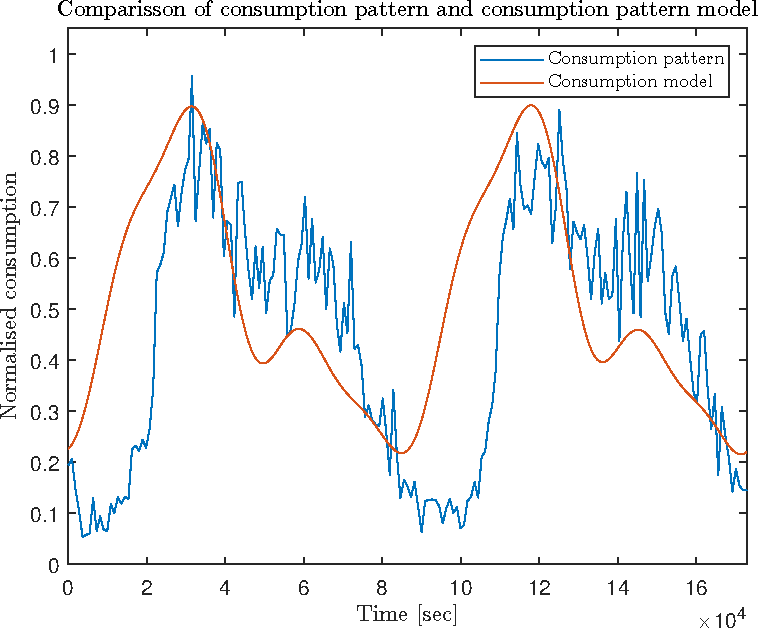
\includegraphics[width=0.6\textwidth]{Topics/KalmanEstimator/Graphics/Comparisson.pdf}
			\caption{Comparison of raw historical data, and model}
			\label{fig:Comparison}
		\end{figure}
	\begin{itemize}
		\item The model follows the visual trend in real data.
	\end{itemize}	
	\end{frame}

\begin{frame}{The Kalman Filter}
	\textbf{Considerations when designing the KF.}
	\begin{itemize}
		\item Stiffness of the filter
	\end{itemize}
\end{frame}